% This file was created by matplotlib2tikz v0.5.7.
% The lastest updates can be retrieved from
% 
% https://github.com/nschloe/matplotlib2tikz
% 
% where you can also submit bug reports and leavecomments.
% 
\documentclass[tikz]{standalone}
\usepackage[utf8]{inputenc}
\usepackage{fontspec}
\usepackage{pgfplots}
\begin{document}
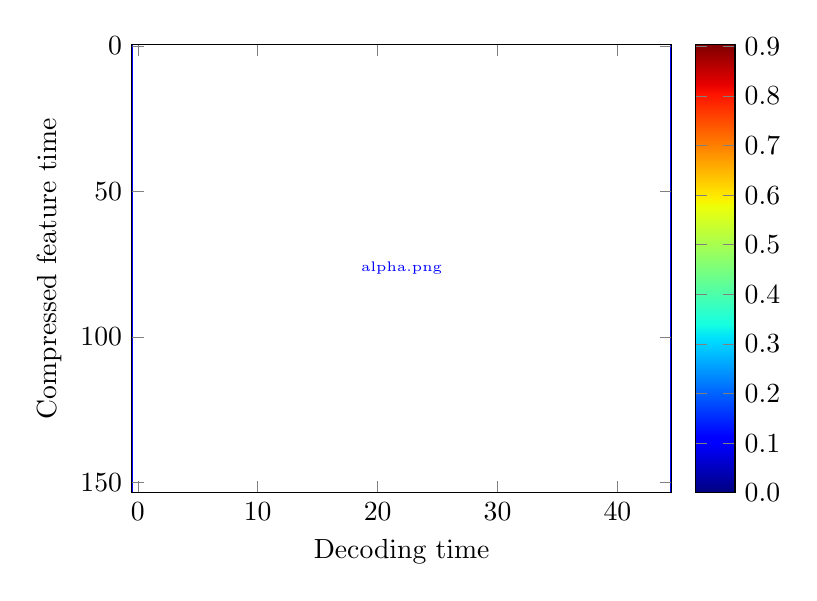
\begin{tikzpicture}


\begin{axis}[
%height = 30cm,
%width = 35cm,
xmin=-0.5, xmax=44.5,
ymin=-0.5, ymax=153.5,
y dir=reverse,
axis on top,
xlabel={Decoding time},
ylabel={Compressed feature time},
%xtick={0,1,2,3,4,5,6,7,8,9,10,11,12,13,14,15,16,17,18,19,20,21,22,23,24,25,26,27,28,29,30,31,32,33,34,35,36,37,38,39,40,41,42,43,44},
%xticklabels={<sos>,sil,hh,ih,f,sil,k,er,r,ow,ow,sil,sil,t,ah,m,aa,hh,hh,ae,v,er,r,r,n,n,sil,f,er,er,m,iy,iy,iy,iy,iy,iy,iy,iy,sil,sil,t,uw,sil,<eos>},
colorbar,
colormap={mymap}{[1pt]
  rgb(0pt)=(0,0,0.5);
  rgb(22pt)=(0,0,1);
  rgb(25pt)=(0,0,1);
  rgb(68pt)=(0,0.86,1);
  rgb(70pt)=(0,0.9,0.967741935483871);
  rgb(75pt)=(0.0806451612903226,1,0.887096774193548);
  rgb(128pt)=(0.935483870967742,1,0.0322580645161291);
  rgb(130pt)=(0.967741935483871,0.962962962962963,0);
  rgb(132pt)=(1,0.925925925925926,0);
  rgb(178pt)=(1,0.0740740740740741,0);
  rgb(182pt)=(0.909090909090909,0,0);
  rgb(200pt)=(0.5,0,0)
},
point meta min=0,
point meta max=0.904238343238831,
colorbar style={ytick={0,0.1,0.2,0.3,0.4,0.5,0.6,0.7,0.8,0.9},yticklabels={0.0,0.1,0.2,0.3,0.4,0.5,0.6,0.7,0.8,0.9}}
]
\addplot graphics [includegraphics cmd=\pgfimage,xmin=-0.5, xmax=44.5, ymin=153.5, ymax=-0.5] {alpha.png};
\end{axis}

\end{tikzpicture}
\end{document}
